\section{Integration Strategy}

\subsection{Entry Criteria}
\todo{da rivedere, guarda keep}
The following conditions have to be verified before entering the integration testing phase in order for it to produce meaningful results.\\
All of the components of the PowerEnJoy system must have passed unit testing with high percentage of covering, so that it is much likely that any problem discovered by integration testing is actually due to integration problems.

\subsection{Elements to be integrated}
Identify the components to be integrated, refer to your design document to identify such components in a way that is consistent with your design.

\subsection{Integration Testing Strategy}
A Bottom-up approach was chosen because most of the functionalities and the complexity is located in lower level components of our system, hence it is a better choice to test them first and ensure that they work well together before higher level components.

\subsection{Sequence of Component Integration}
Depends on strategy chosen, this is a proposed structure.

\subsubsection{Overall Component Integration Diagram} 
The diagram above shows the needed precedences in the integration phase between the main components of the system.

	\begin{figure}[h]
			\centering
			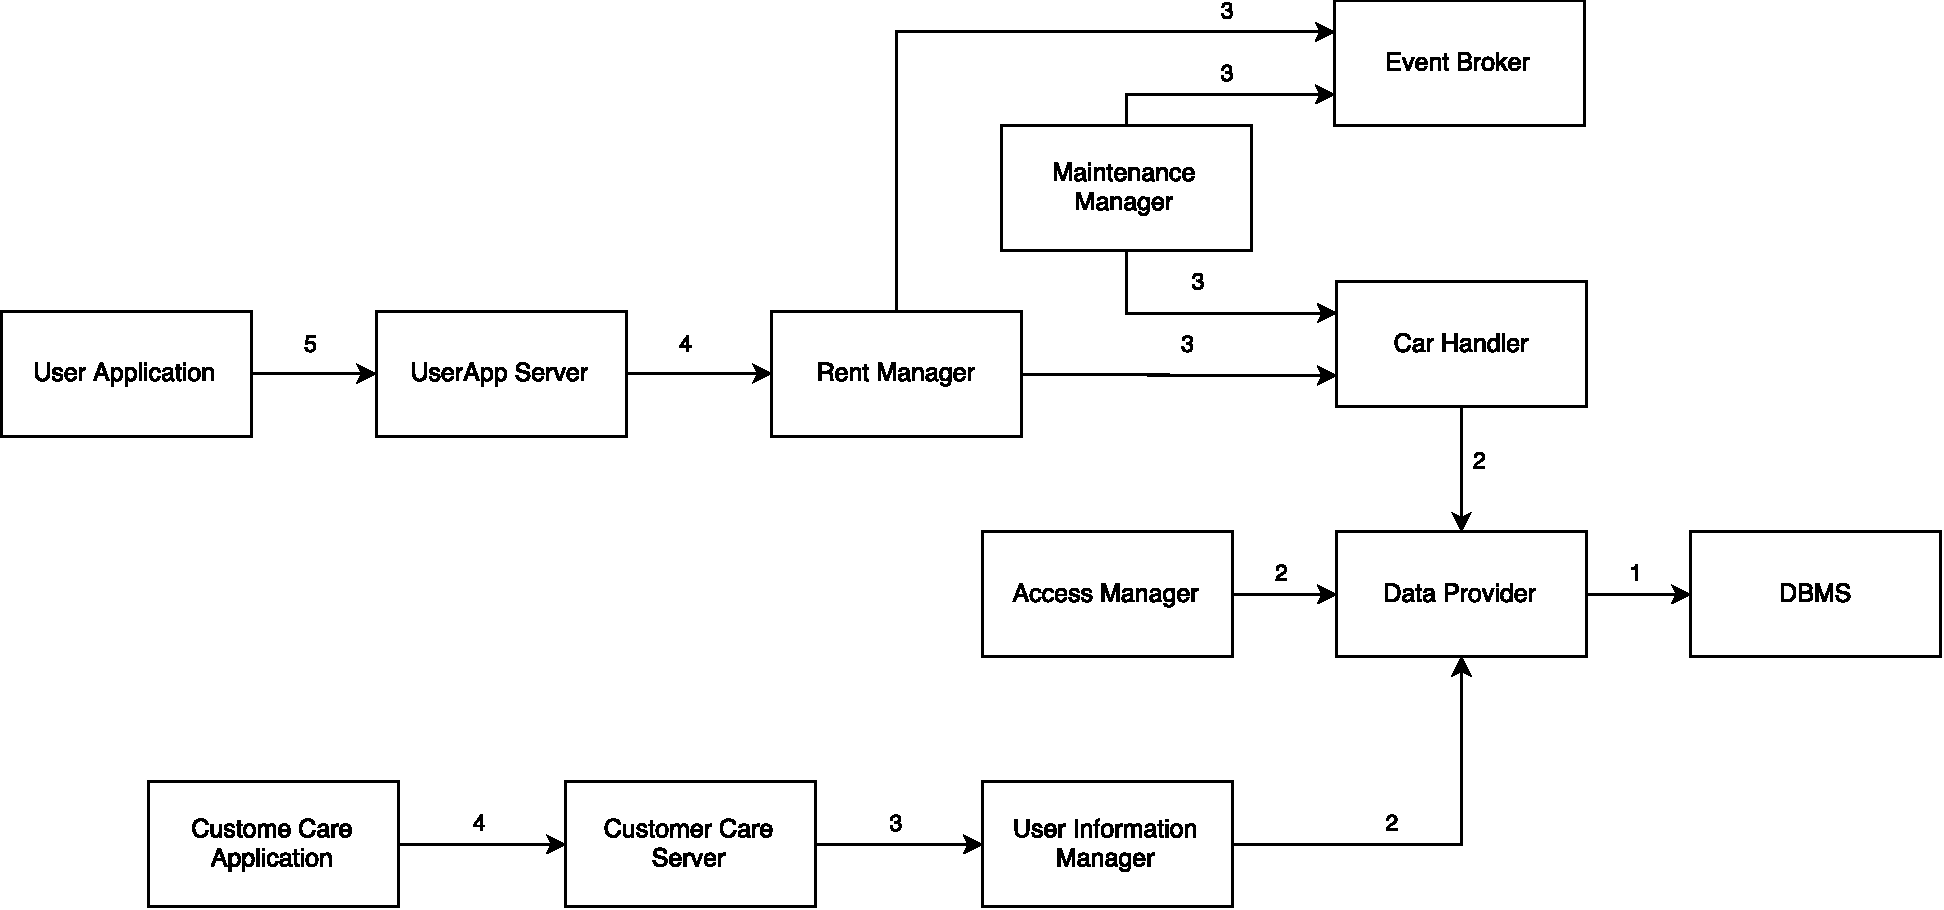
\includegraphics[width=\linewidth]{img/overallIntegration}
			\caption{
				\label{fig:overallIntegration} 
				\emph{Overall Component Integration Diagram}
			}
		\end{figure}

\clearpage

\subsubsection{Unit Testing} 
Fare unit test con attenzione a queste precedenze nei seguenti componenti.
\todo{tradurre e sistemare}

\paragraph{RentManager} 
The diagram above shows the needed precedences in the integration phase inside the \emph{RentManager} component.
\paragraph{}

		\begin{figure}[h]
			\centering
			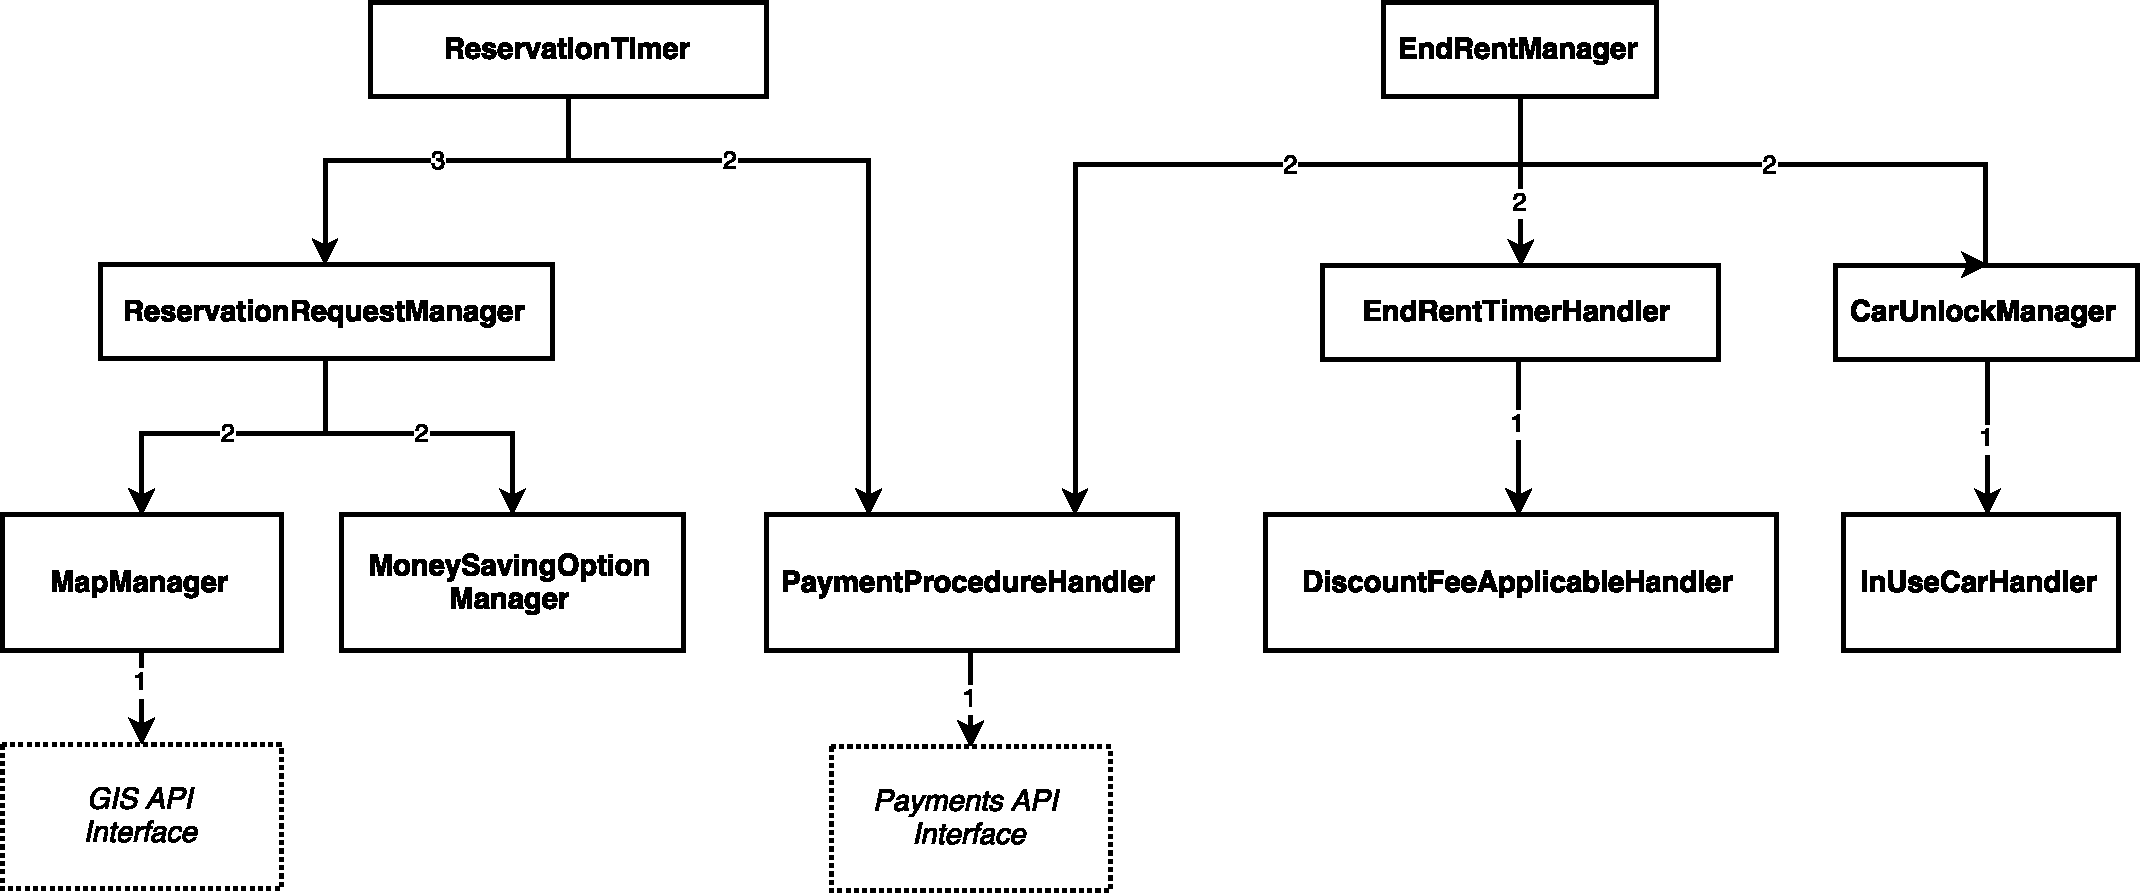
\includegraphics[width=\linewidth]{img/rentManagerIntegration}
			\caption{
				\label{fig:rentManagerIntegration} 
				\emph{RentManager integration}
			}
		\end{figure}
		
\paragraph{MaintenanceManager} 
The diagram above shows the needed precedences in the integration phase inside the \emph{MaintenanceManager} component.
\paragraph{}

		\begin{figure}[h]
			\centering
			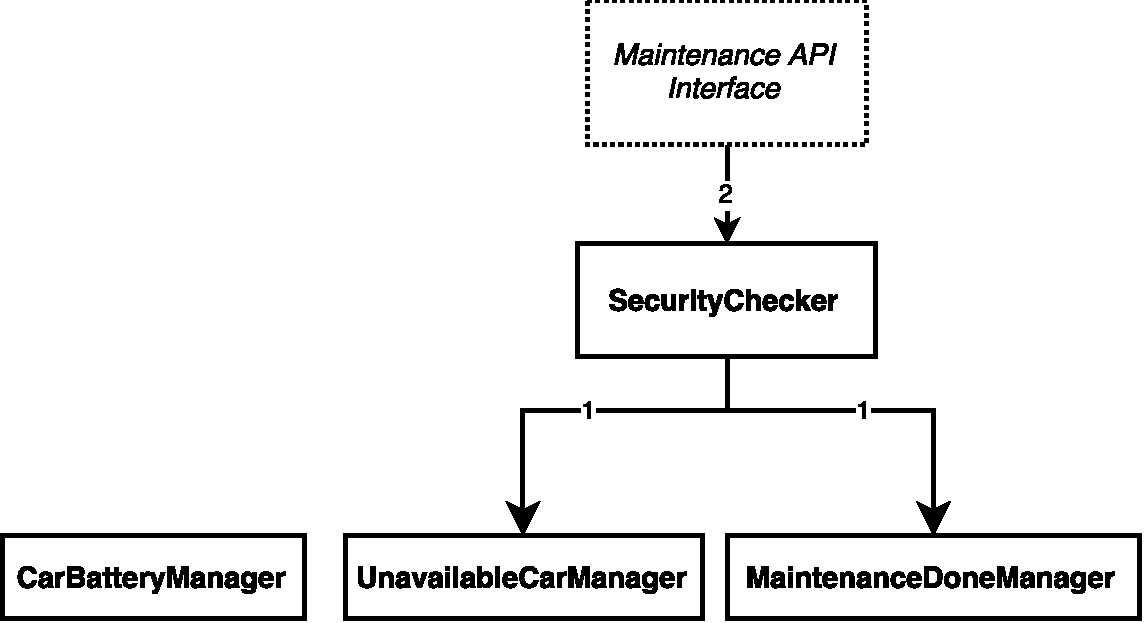
\includegraphics[width=\linewidth]{img/maintenanceIntegration}
			\caption{
				\label{fig:maintenanceIntegration} 
				\emph{MaintenanceManager integration}
			}
		\end{figure}
		
\paragraph{UserInformationManager} 
The diagram above shows the needed precedences in the integration phase inside the \emph{UserInformationManager} component.
\paragraph{}

		\begin{figure}[h]
			\centering
			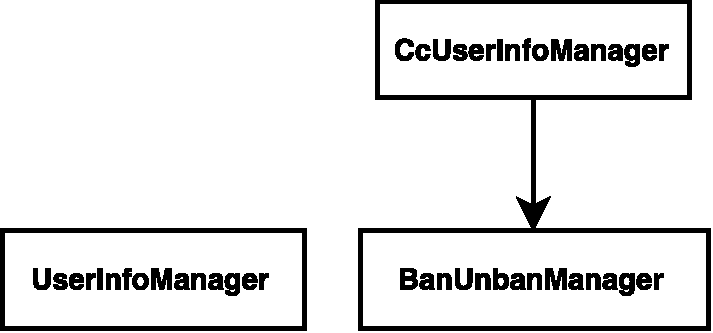
\includegraphics[width=0.6\linewidth]{img/userIntegration}
			\caption{
				\label{fig:userIntegration} 
				\emph{UserInformationManager integration}
			}
		\end{figure}

\clearpage

\subsubsection{Component Integration}

\paragraph{DataProvider} 
...
\paragraph{}

		\begin{figure}[h]
			\centering
			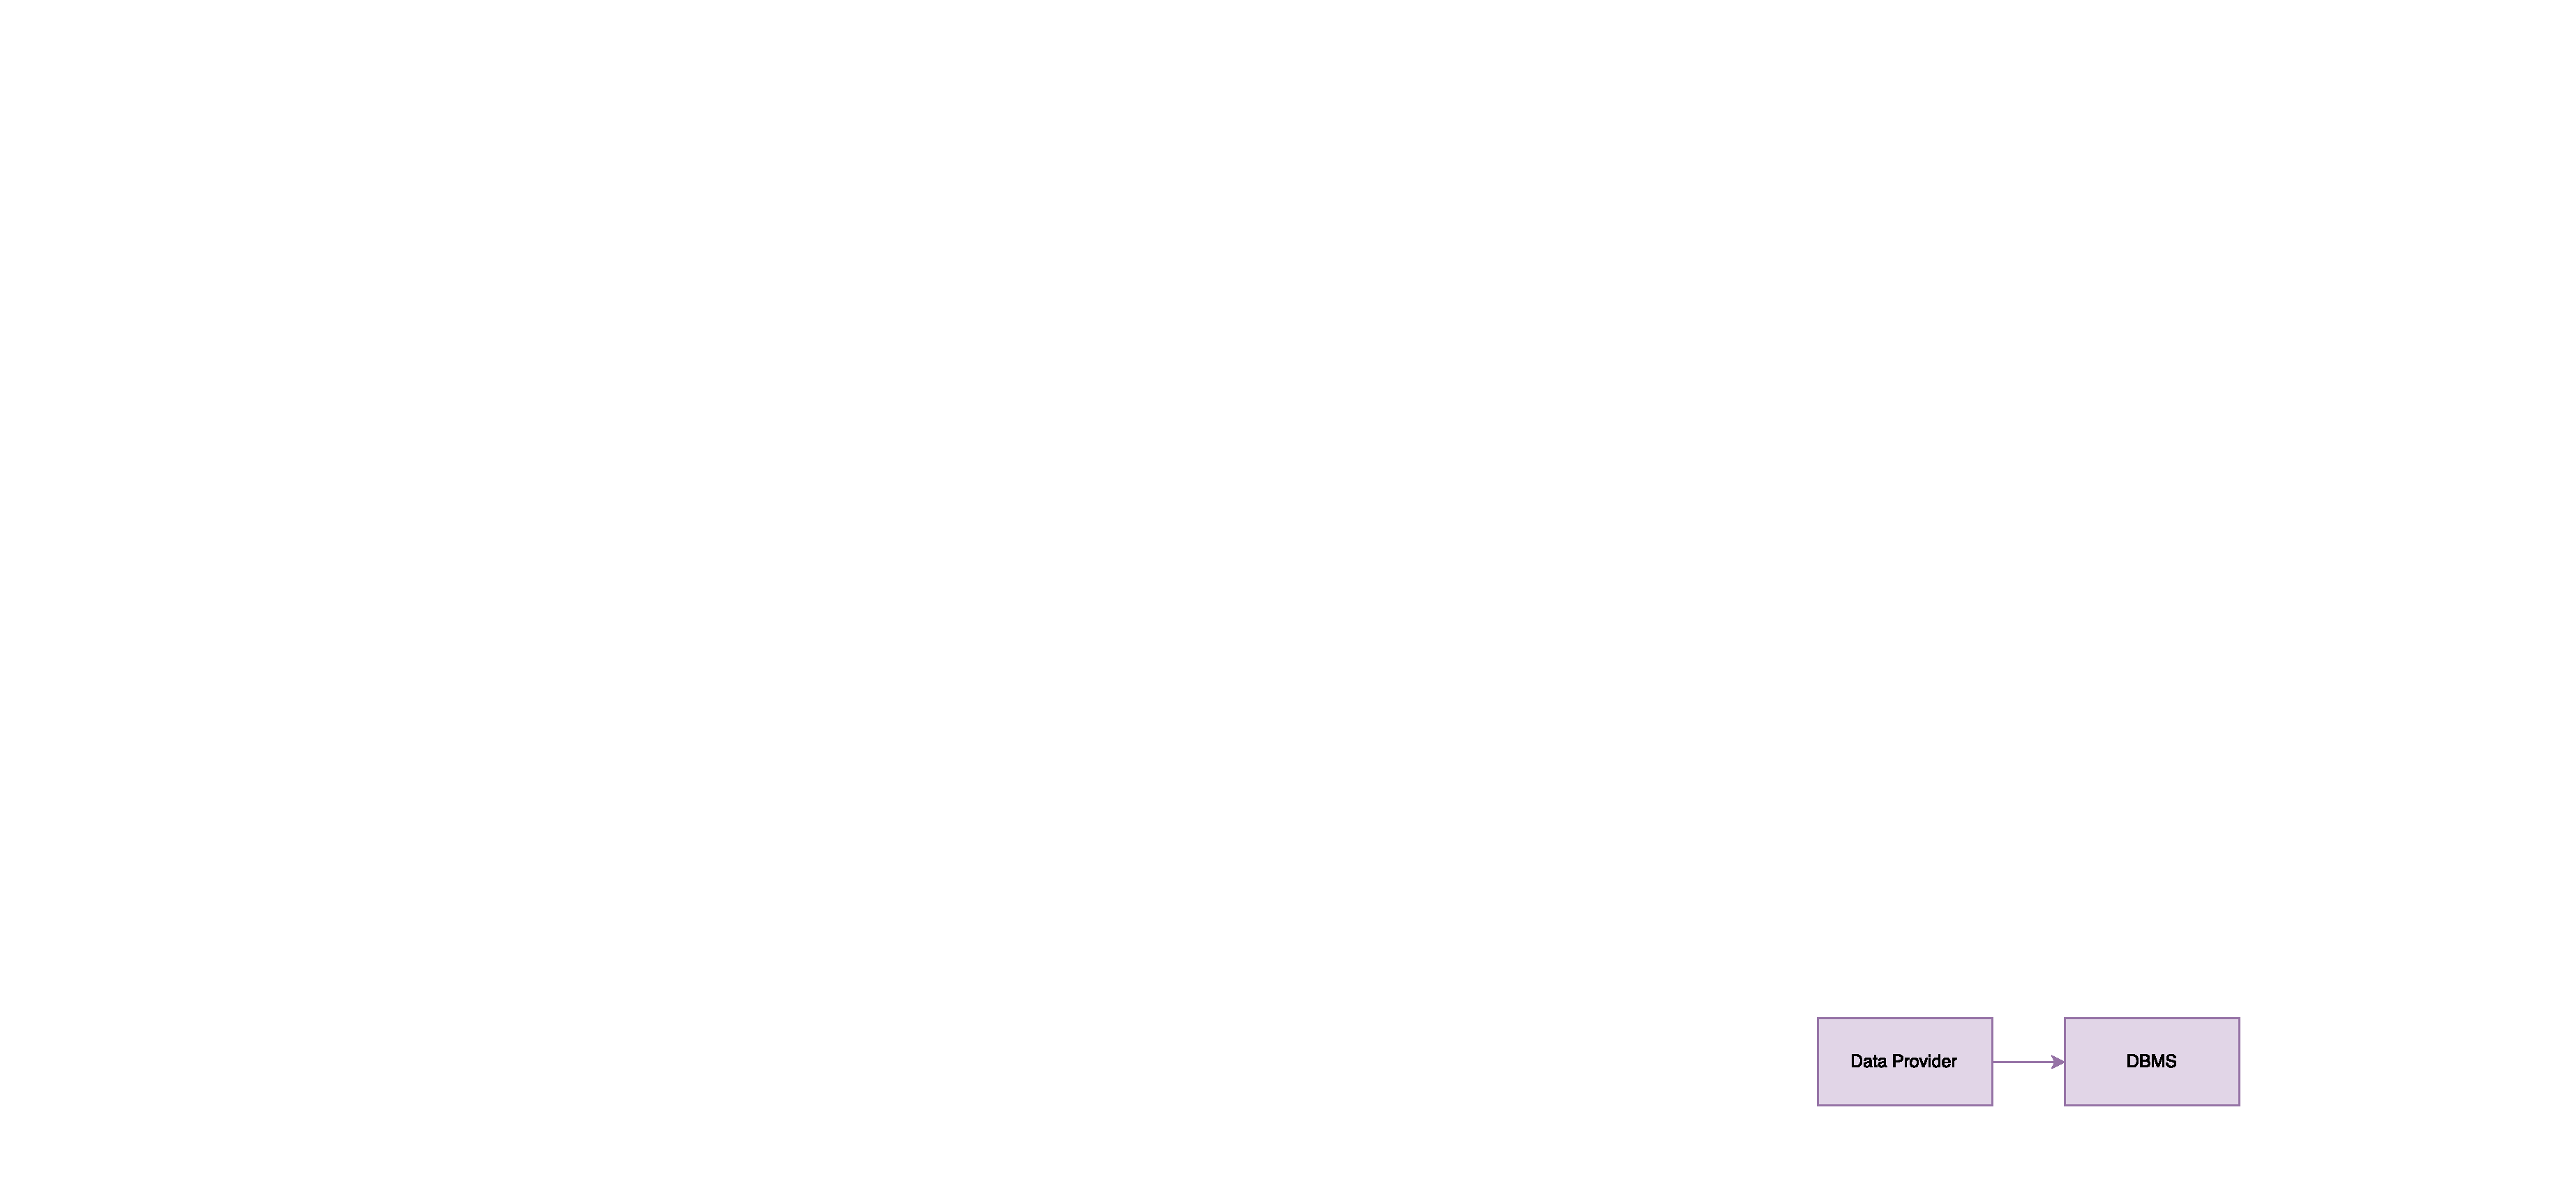
\includegraphics[width=0.6\linewidth]{img/Integration1}
			\caption{
				\label{fig:dataProvider} 
				\emph{DataProvider integration}
			}
		\end{figure}

\paragraph{EventBroker and CarHandler} 
...
\paragraph{}
		
		\begin{figure}[h]
			\centering
			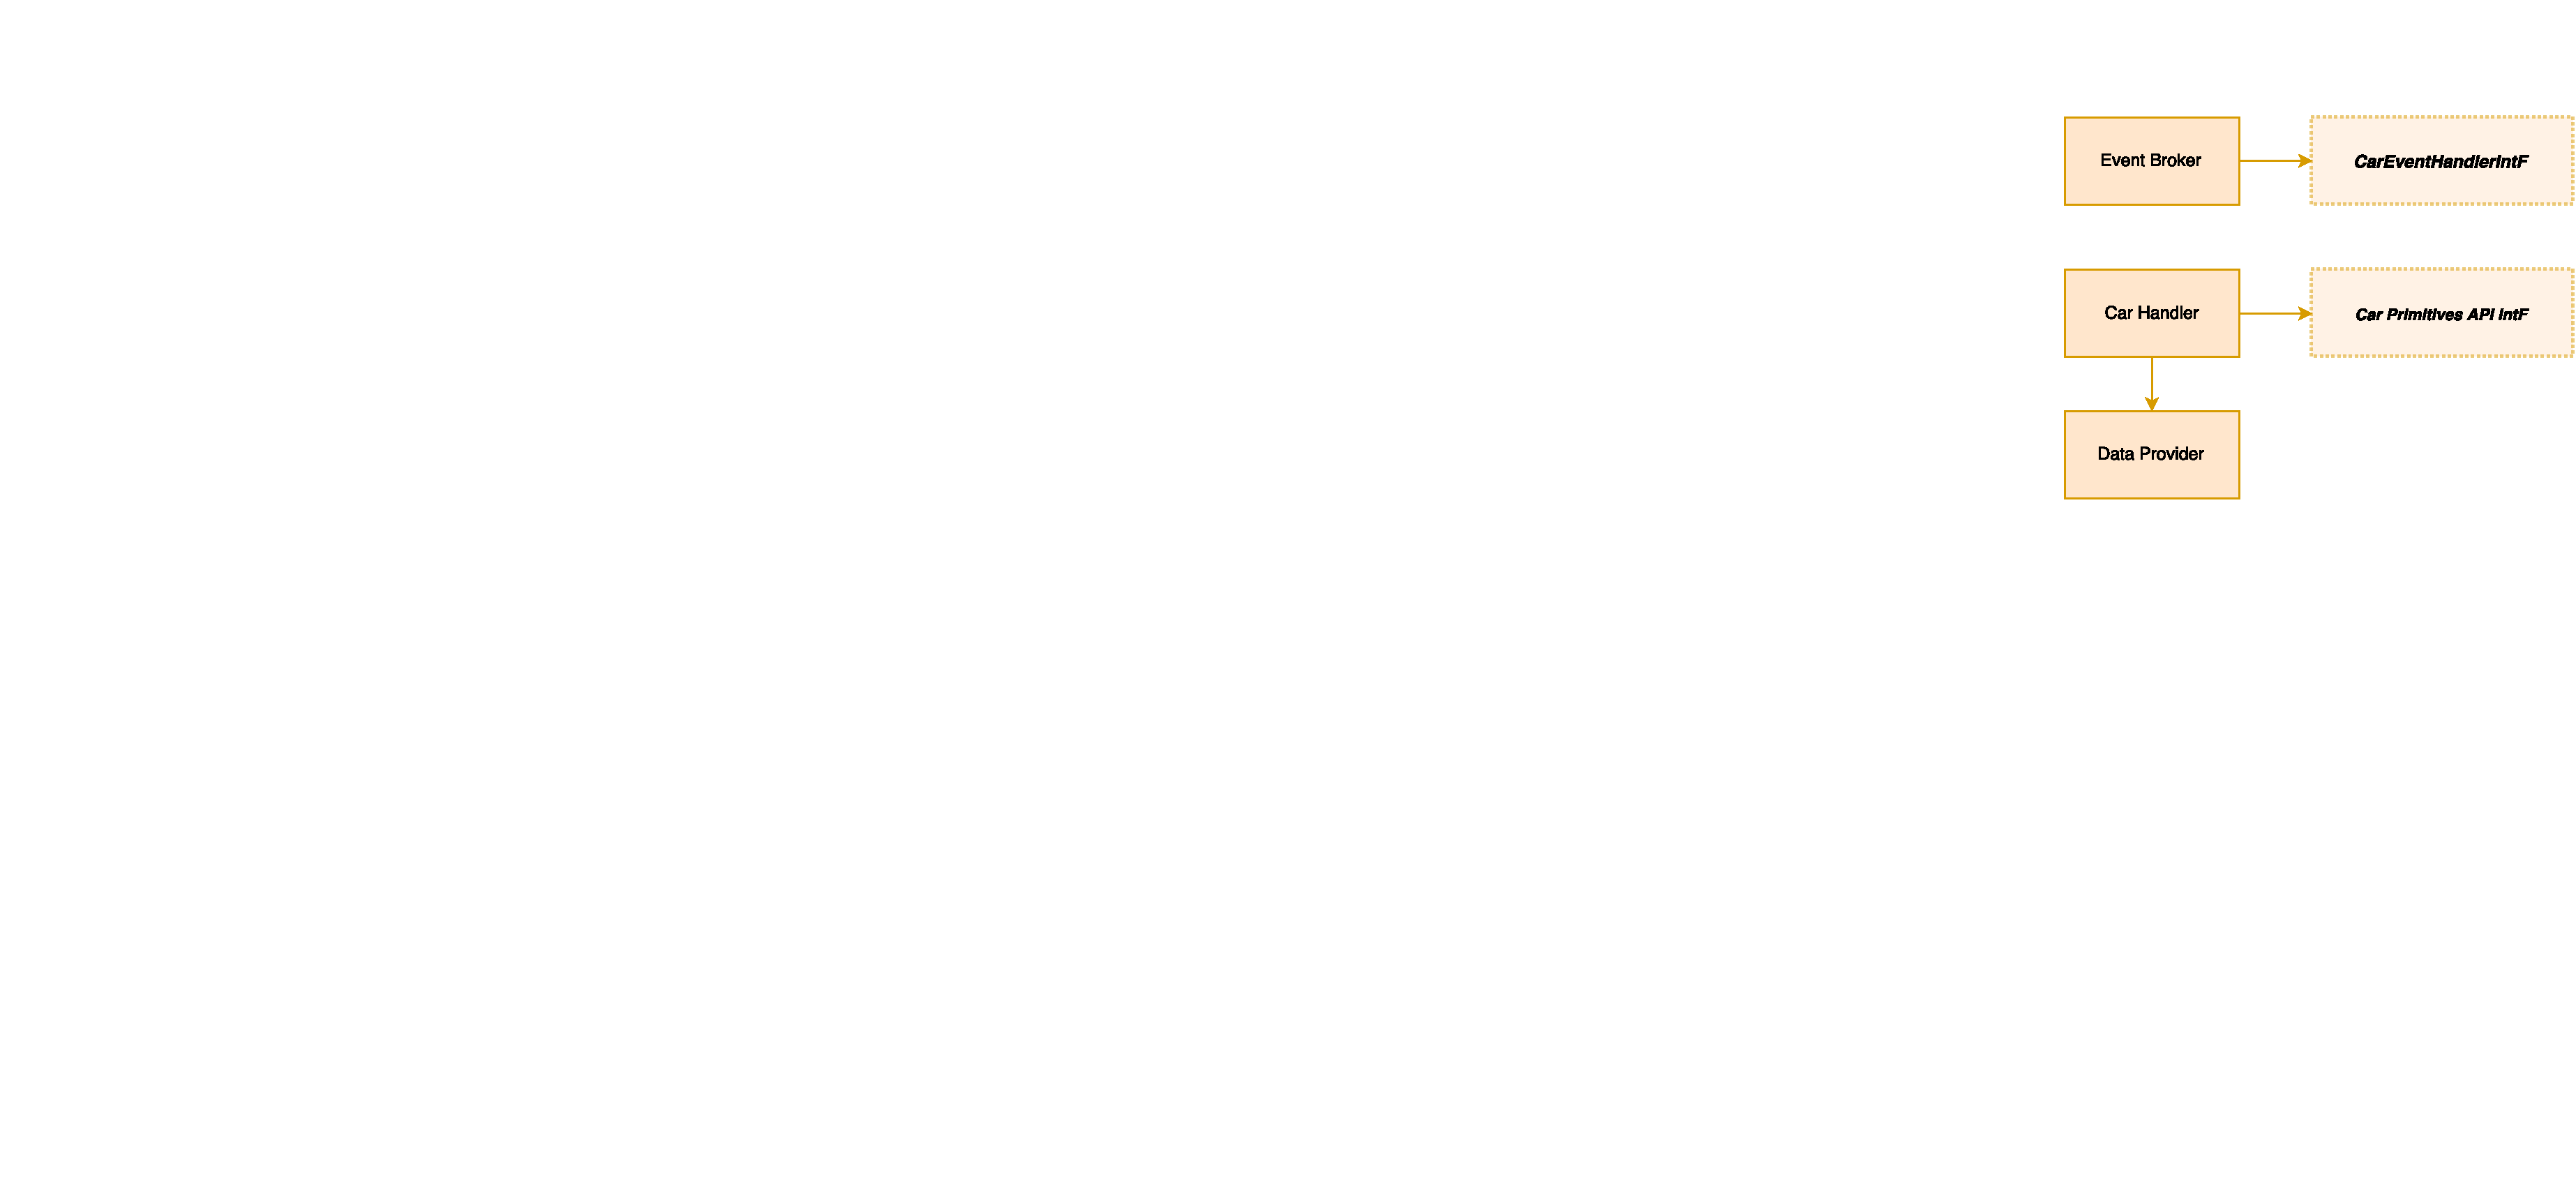
\includegraphics[width=0.6\linewidth]{img/Integration2a}
			\caption{
				\label{fig:eventBrokerCarHandler} 
				\emph{EventBroker and CarHandler integration}
			}
		\end{figure}

\paragraph{UserInformationManager and AccessManager} 
...
\paragraph{}
		
		\begin{figure}[h]
			\centering
			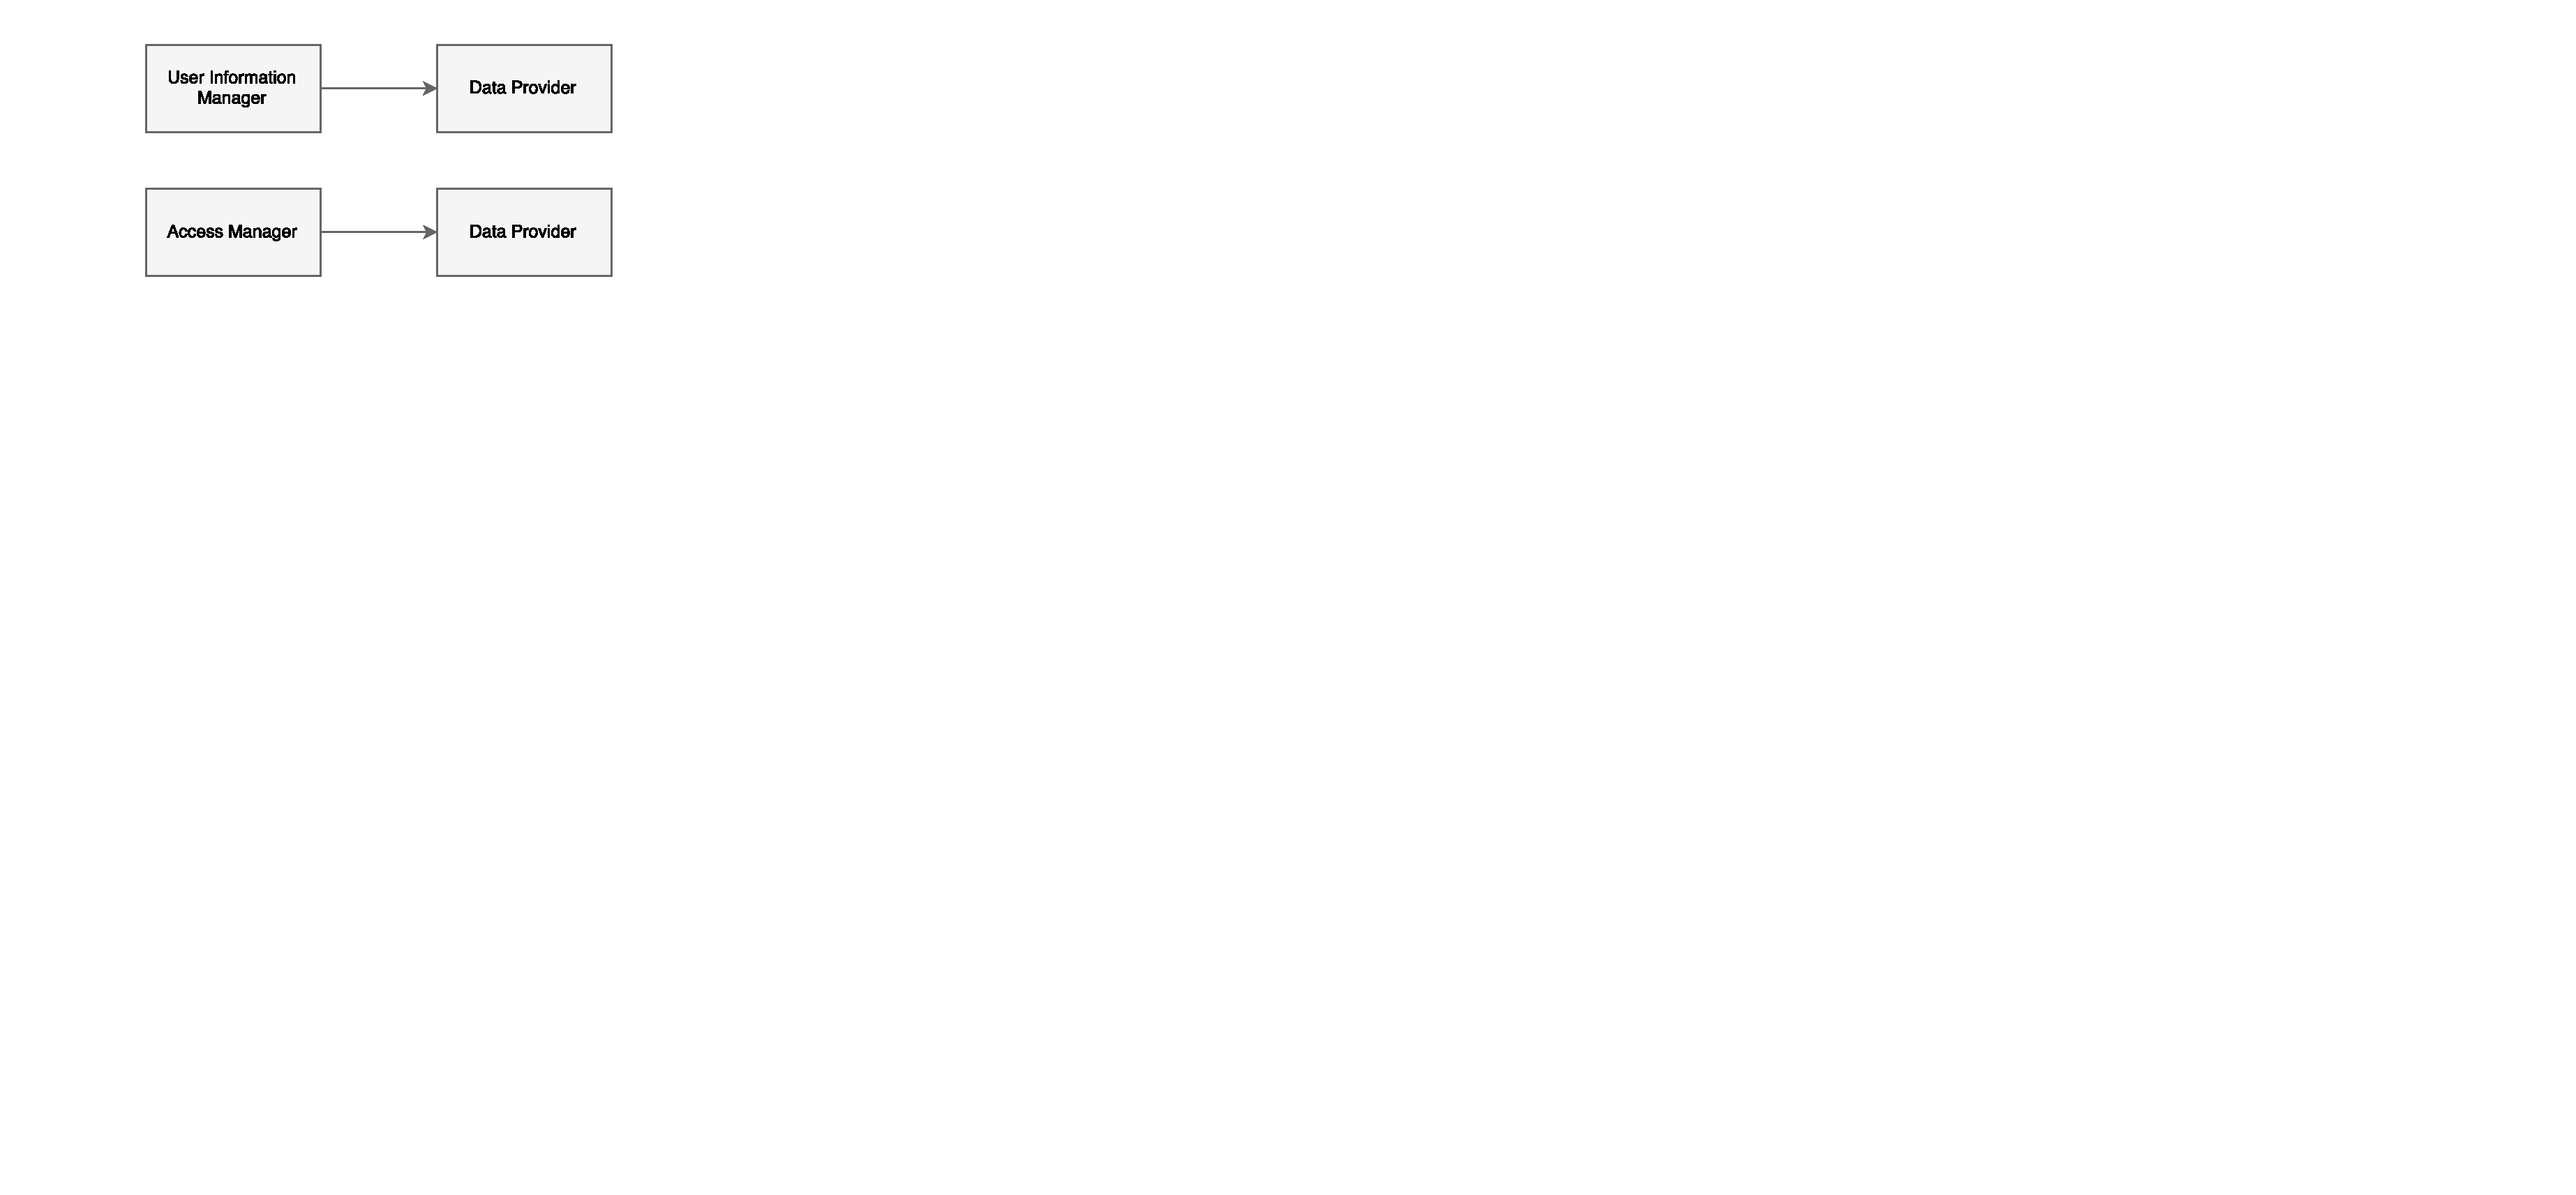
\includegraphics[width=0.6\linewidth]{img/Integration2b}
			\caption{
				\label{fig:userInfoAccessManager} 
				\emph{UserInformationManager and AccessManager integration}
			}
		\end{figure}
		
\paragraph{RentManager} 
...
\paragraph{}
		
		\begin{figure}[h]
			\centering
			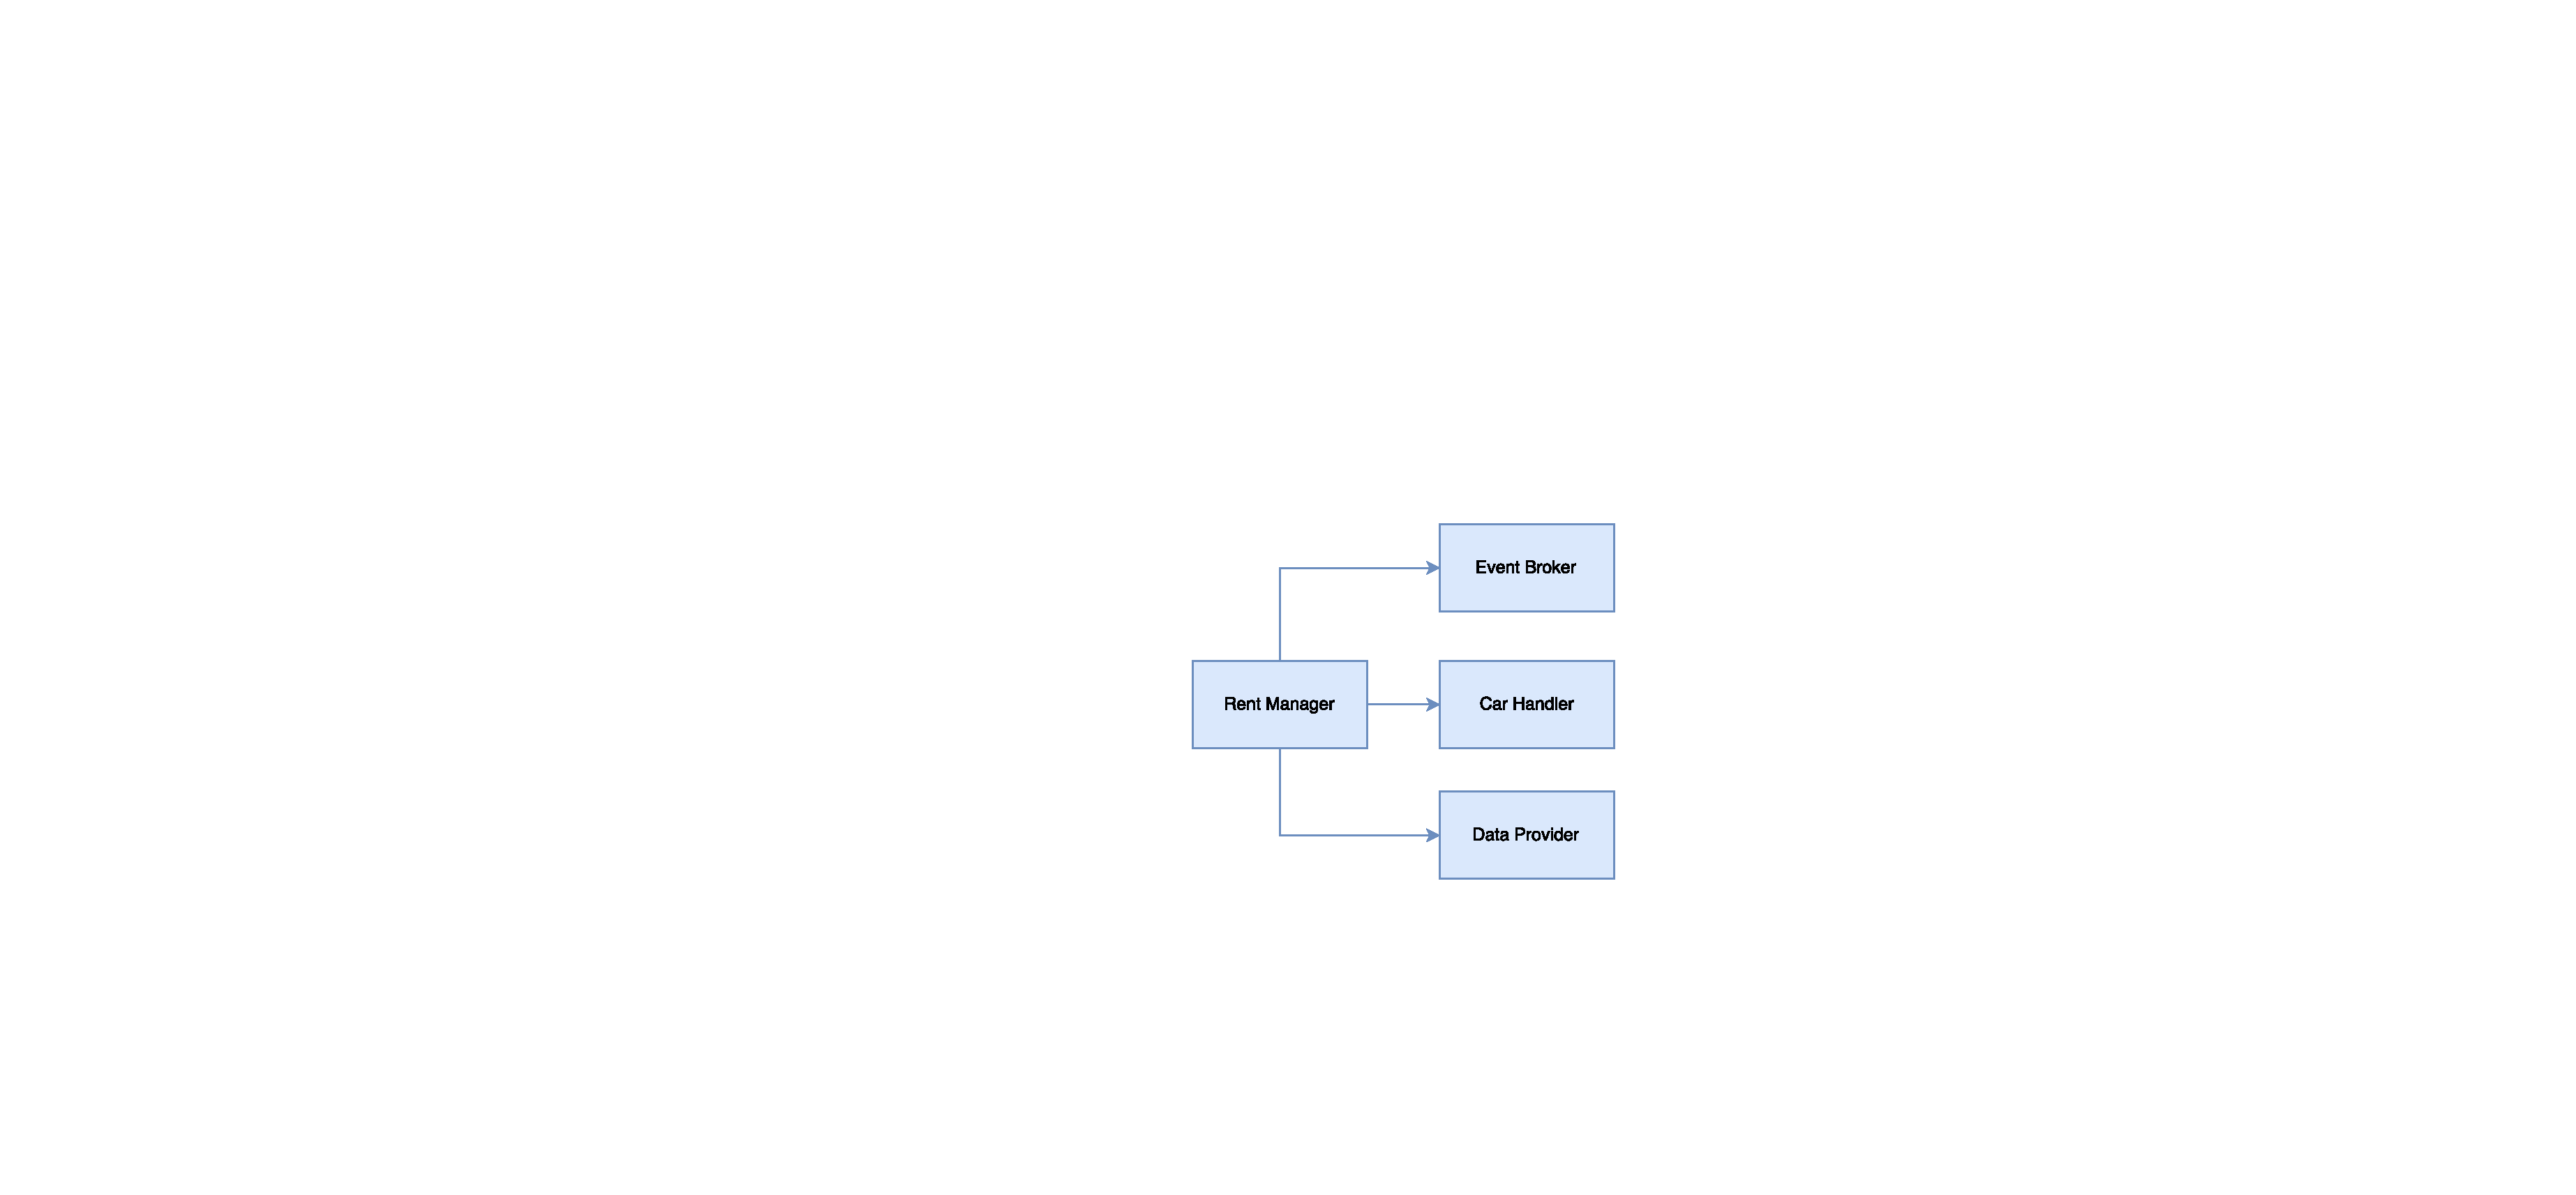
\includegraphics[width=0.8\linewidth]{img/Integration3a}
			\caption{
				\label{fig:rentManager} 
				\emph{RentManager integration}
			}
		\end{figure}

\paragraph{MaintenanceManager} 
...
\paragraph{}
		
		\begin{figure}[h]
			\centering
			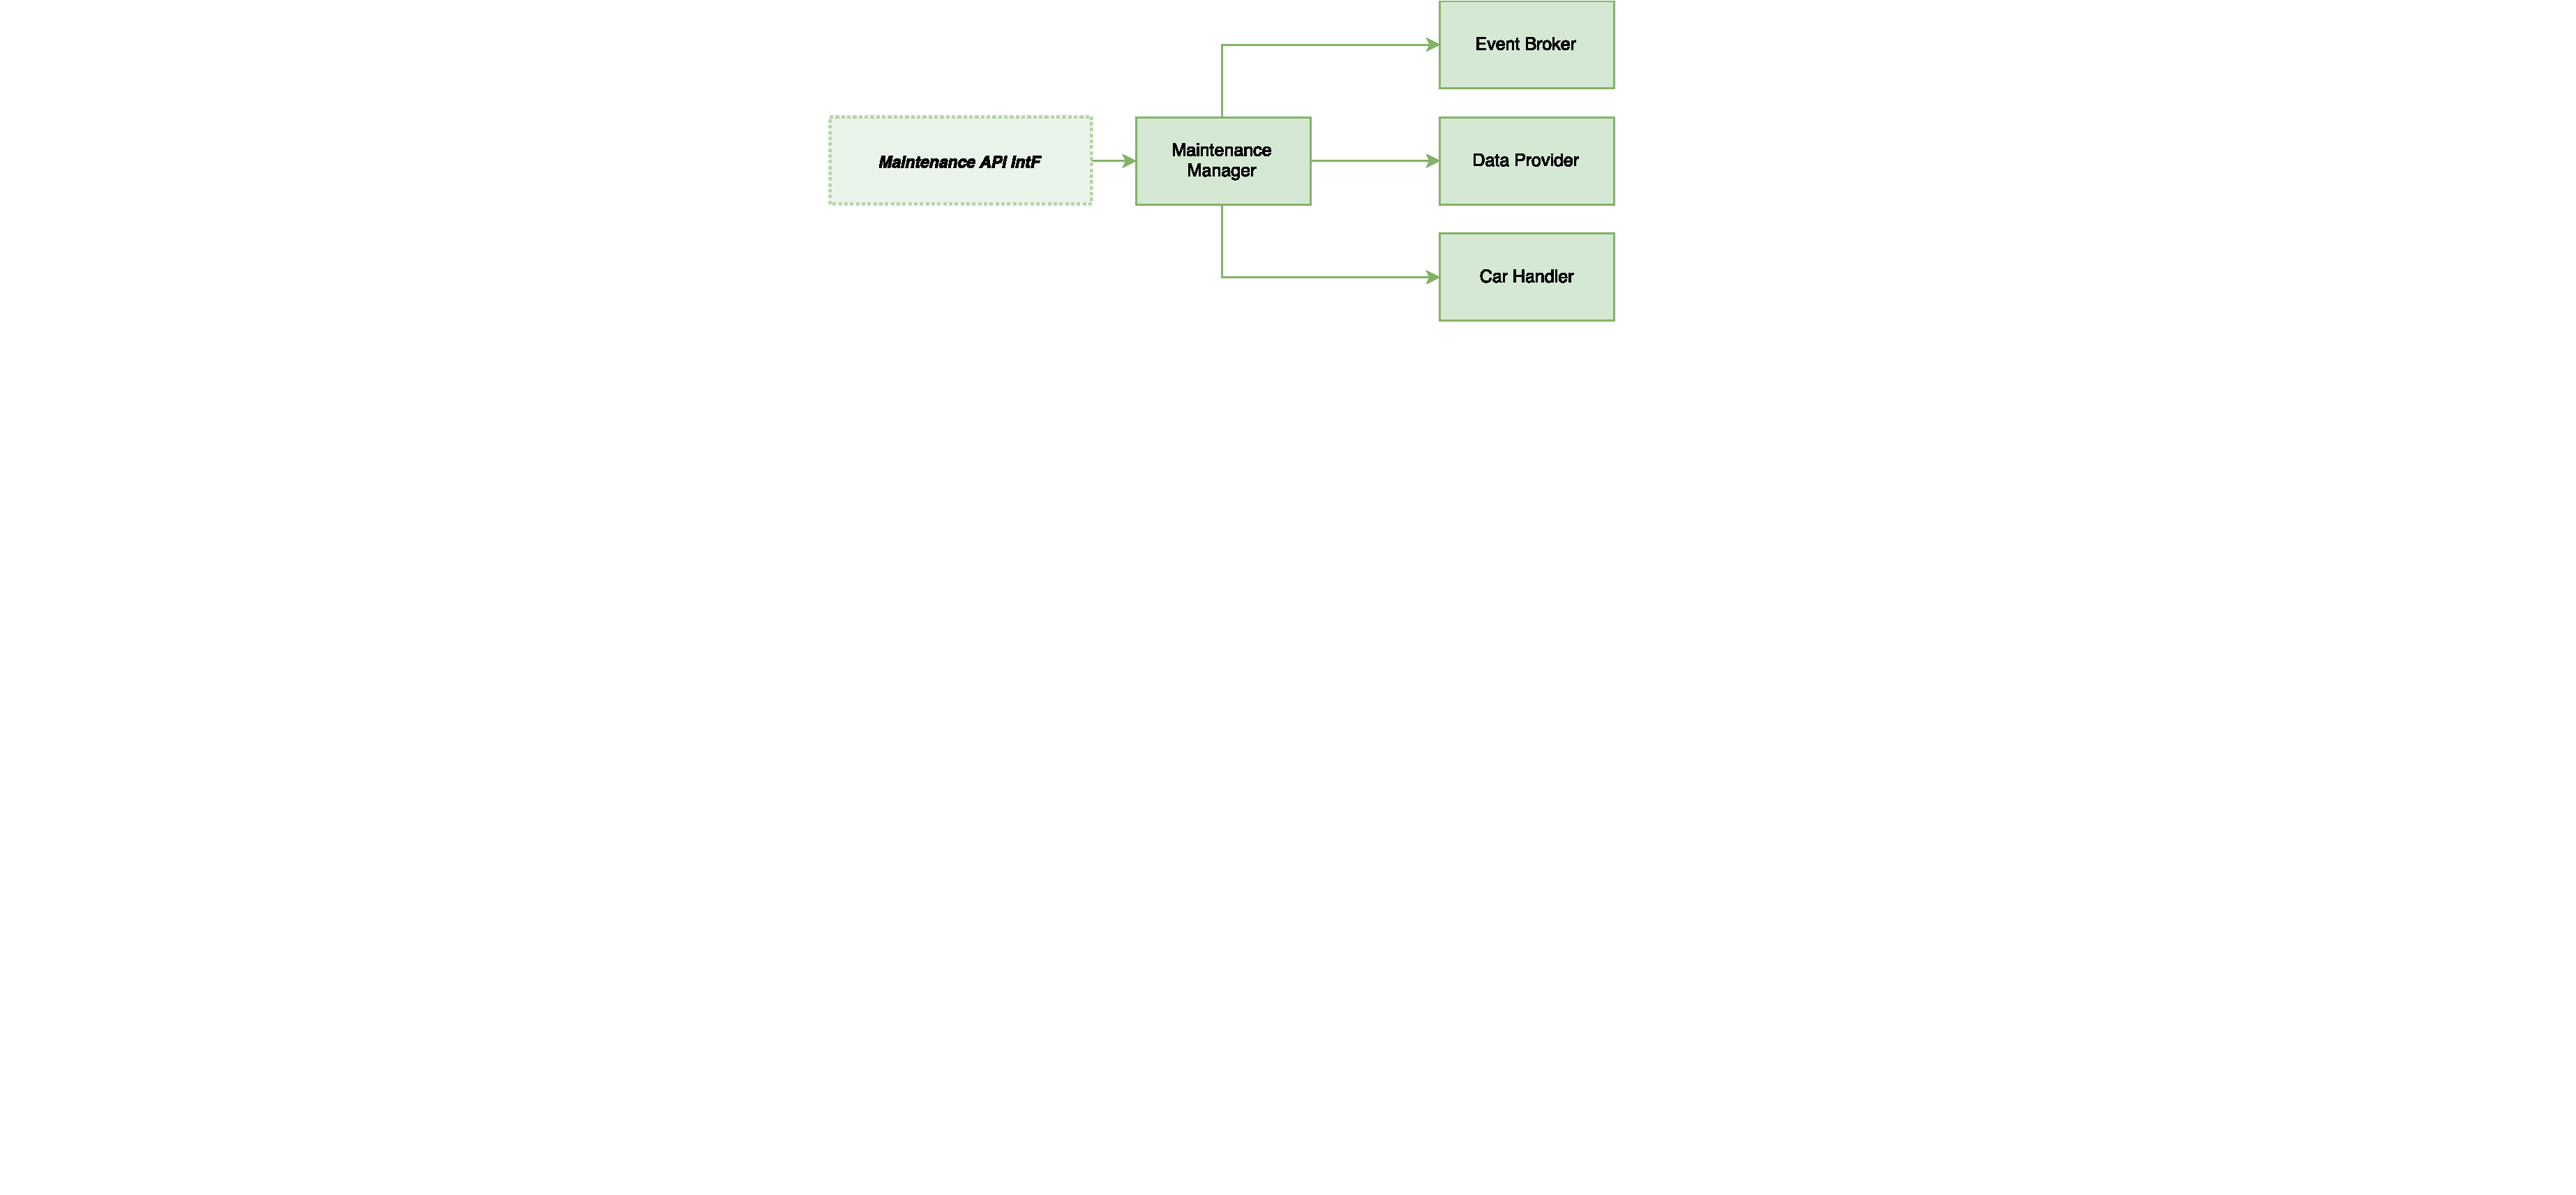
\includegraphics[width=0.8\linewidth]{img/Integration3b}
			\caption{
				\label{fig:maintenanceManager} 
				\emph{MaintenanceManager integration}
			}
		\end{figure}
		
\paragraph{CustomerCare Application and Server} 
...
\paragraph{}
		
		\begin{figure}[h]
			\centering
			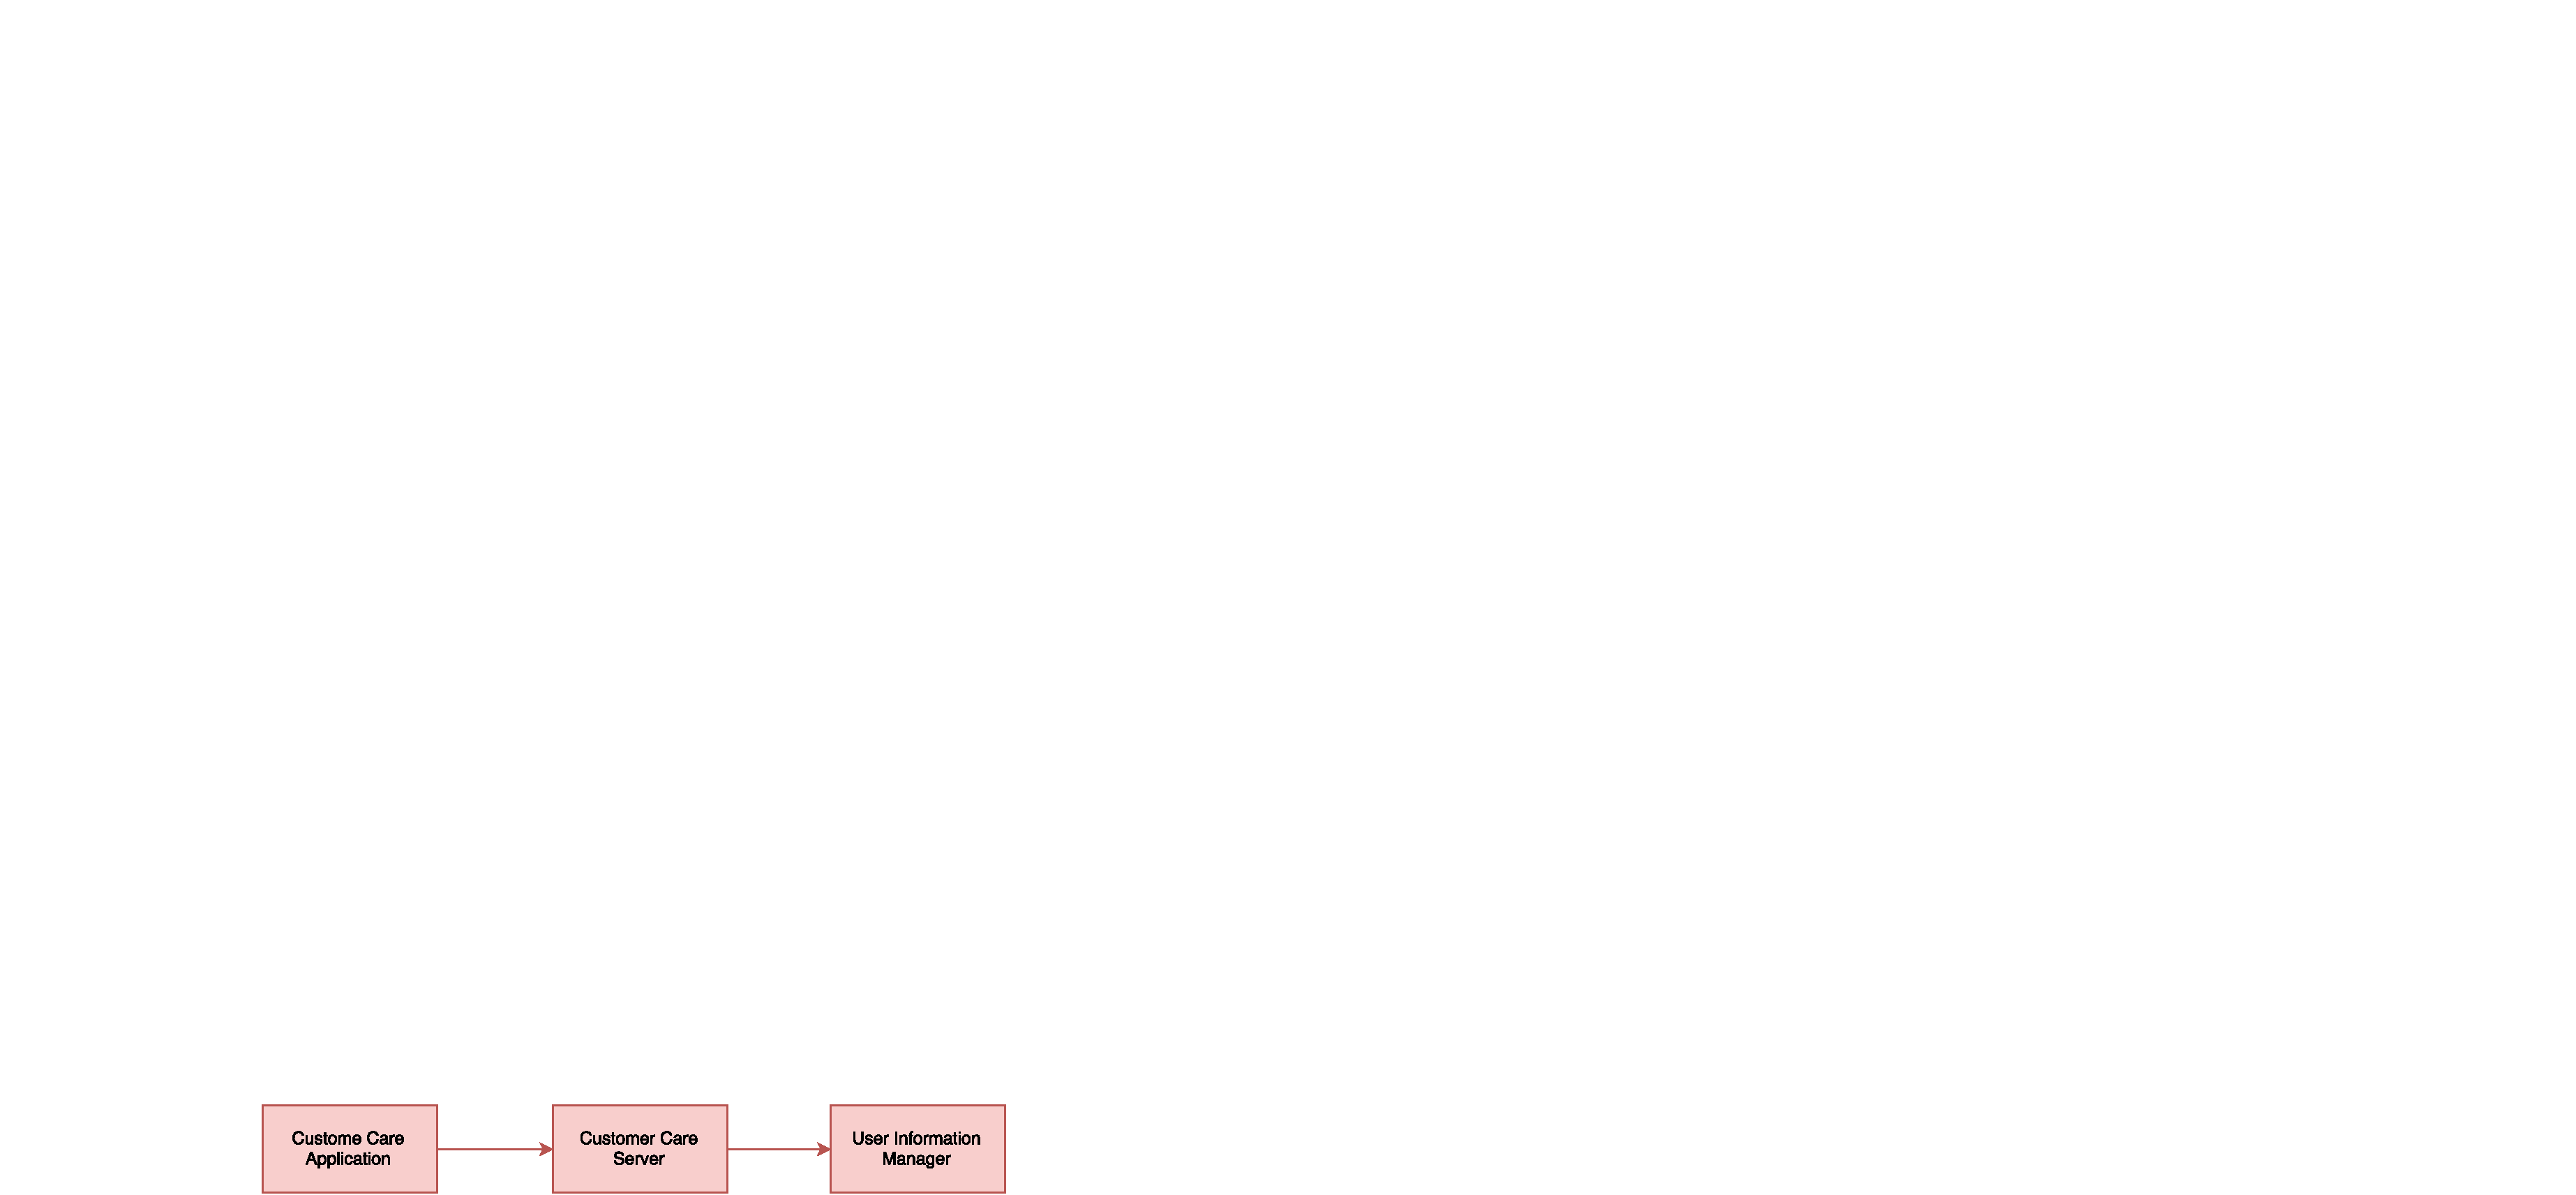
\includegraphics[width=0.8\linewidth]{img/Integration3c}
			\caption{
				\label{fig:ccAppServer} 
				\emph{CustomerCare Application and Server integration}
			}
		\end{figure}
		
\paragraph{User Application and Server} 
...
\paragraph{}
		
		\begin{figure}[h]
			\centering
			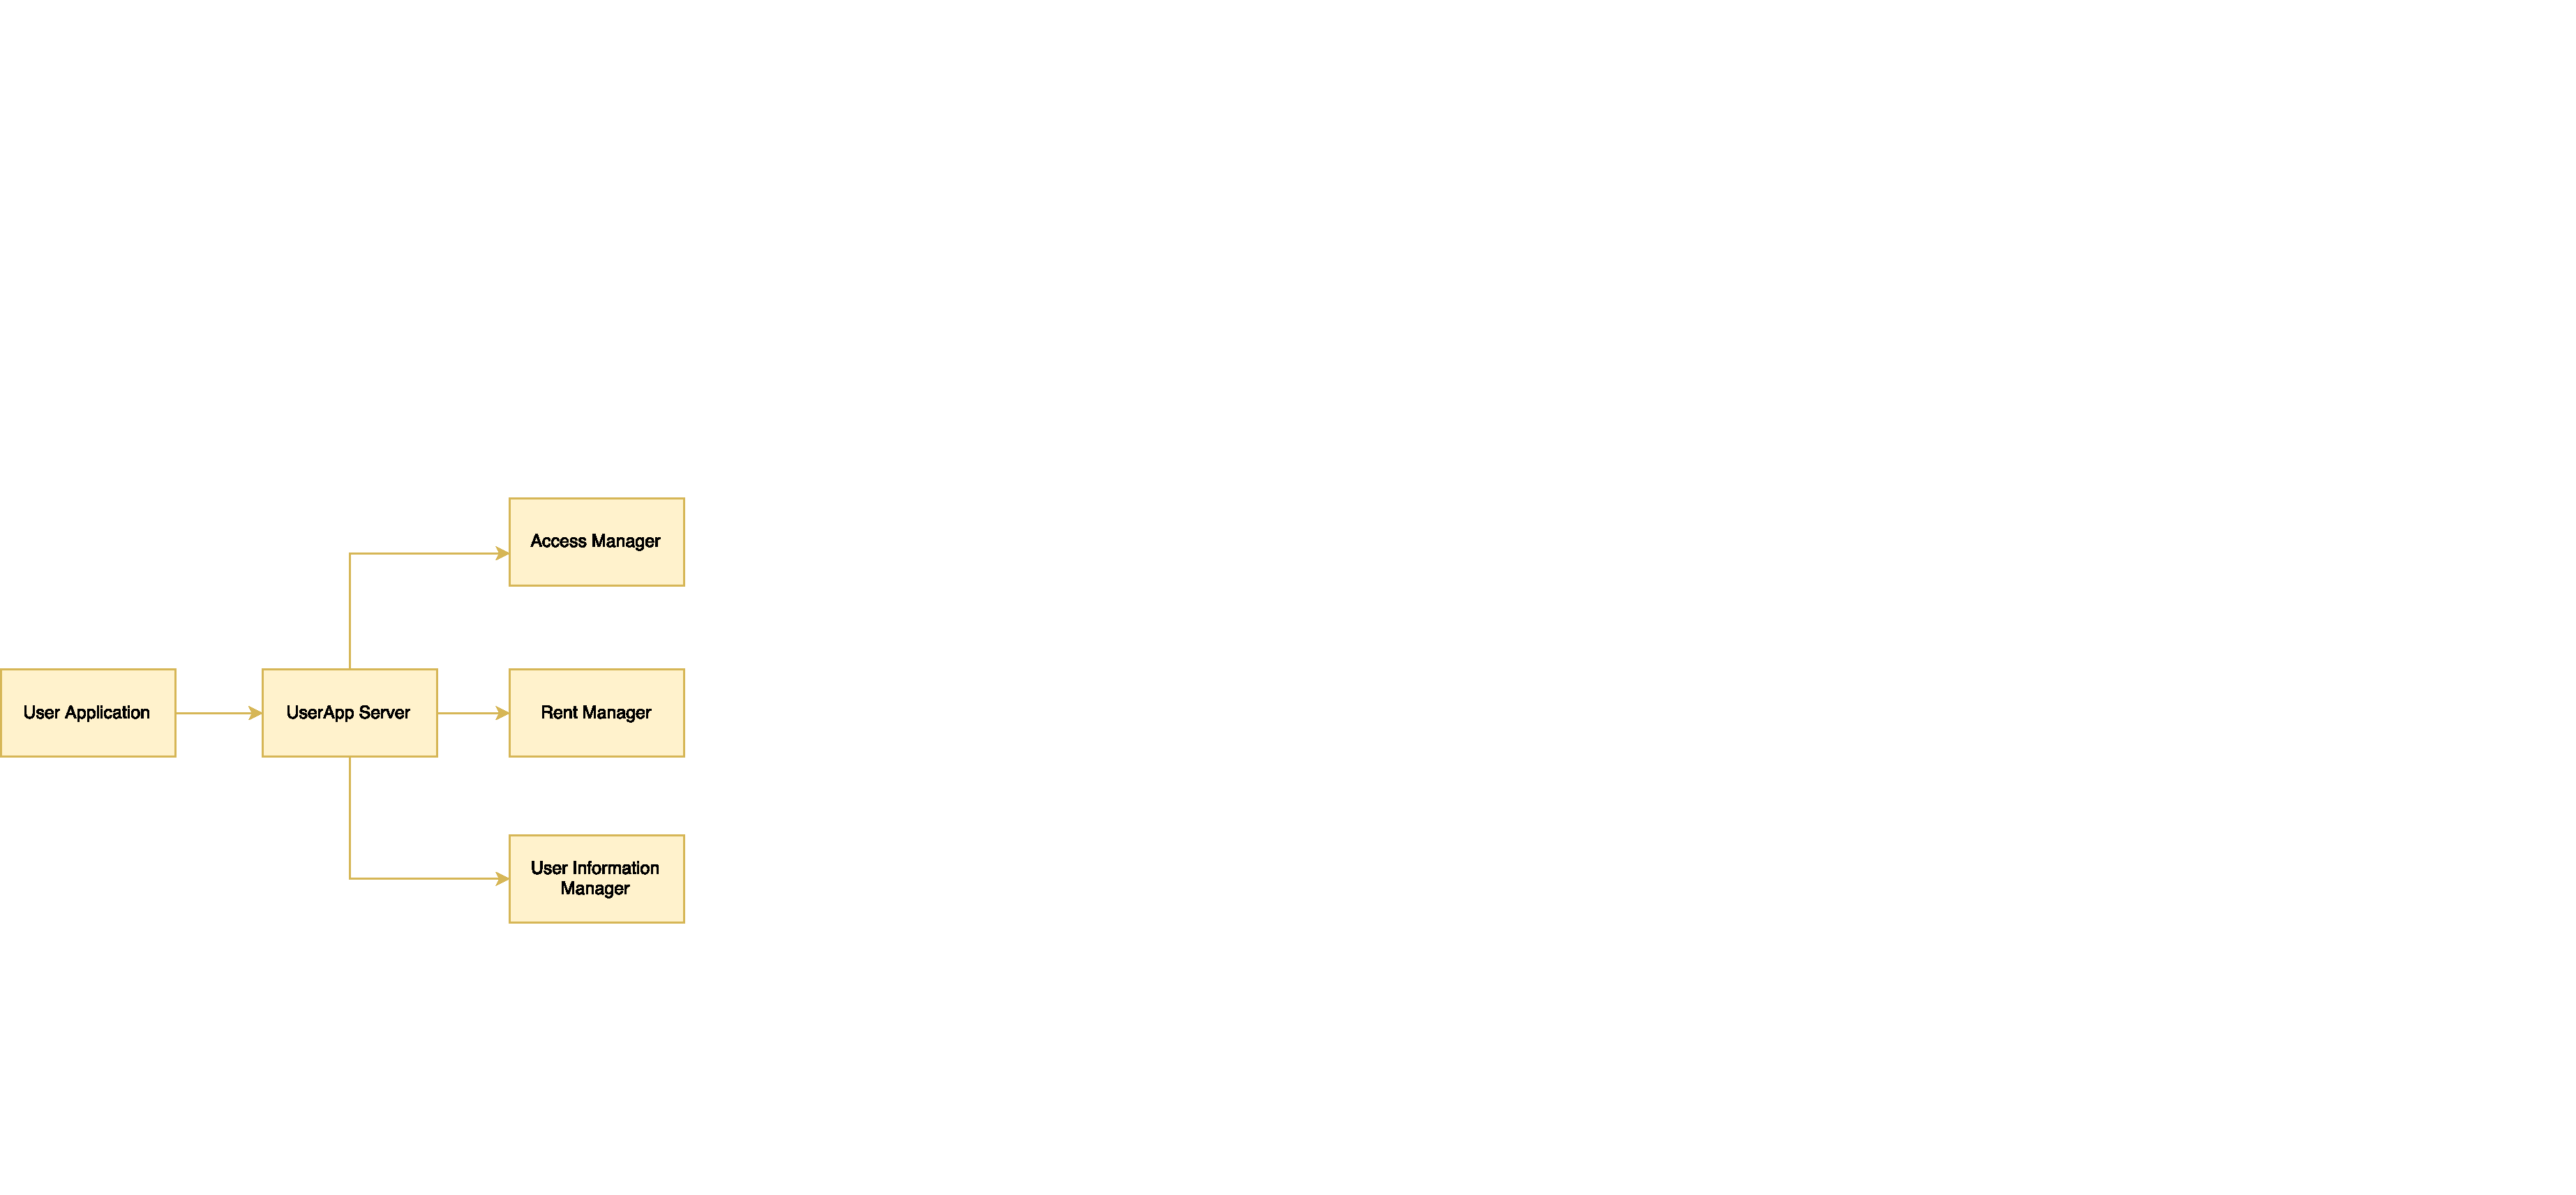
\includegraphics[width=0.8\linewidth]{img/Integration4}
			\caption{
				\label{fig:userAppServer} 
				\emph{User Application and Server integration}
			}
		\end{figure}

\clearpage 

\subsubsection{Subsystem Integration Sequence}

Unisco i sottosistemi del Maintenance (figura \ref{fig:maintenanceManager}), dello User (figura \ref{fig:userAppServer})  e del Customer Care (figura \ref{fig:ccAppServer}) nel sistema finale e testo tutto insieme. \todo{inglese}

	\begin{figure}[h]
			\centering
			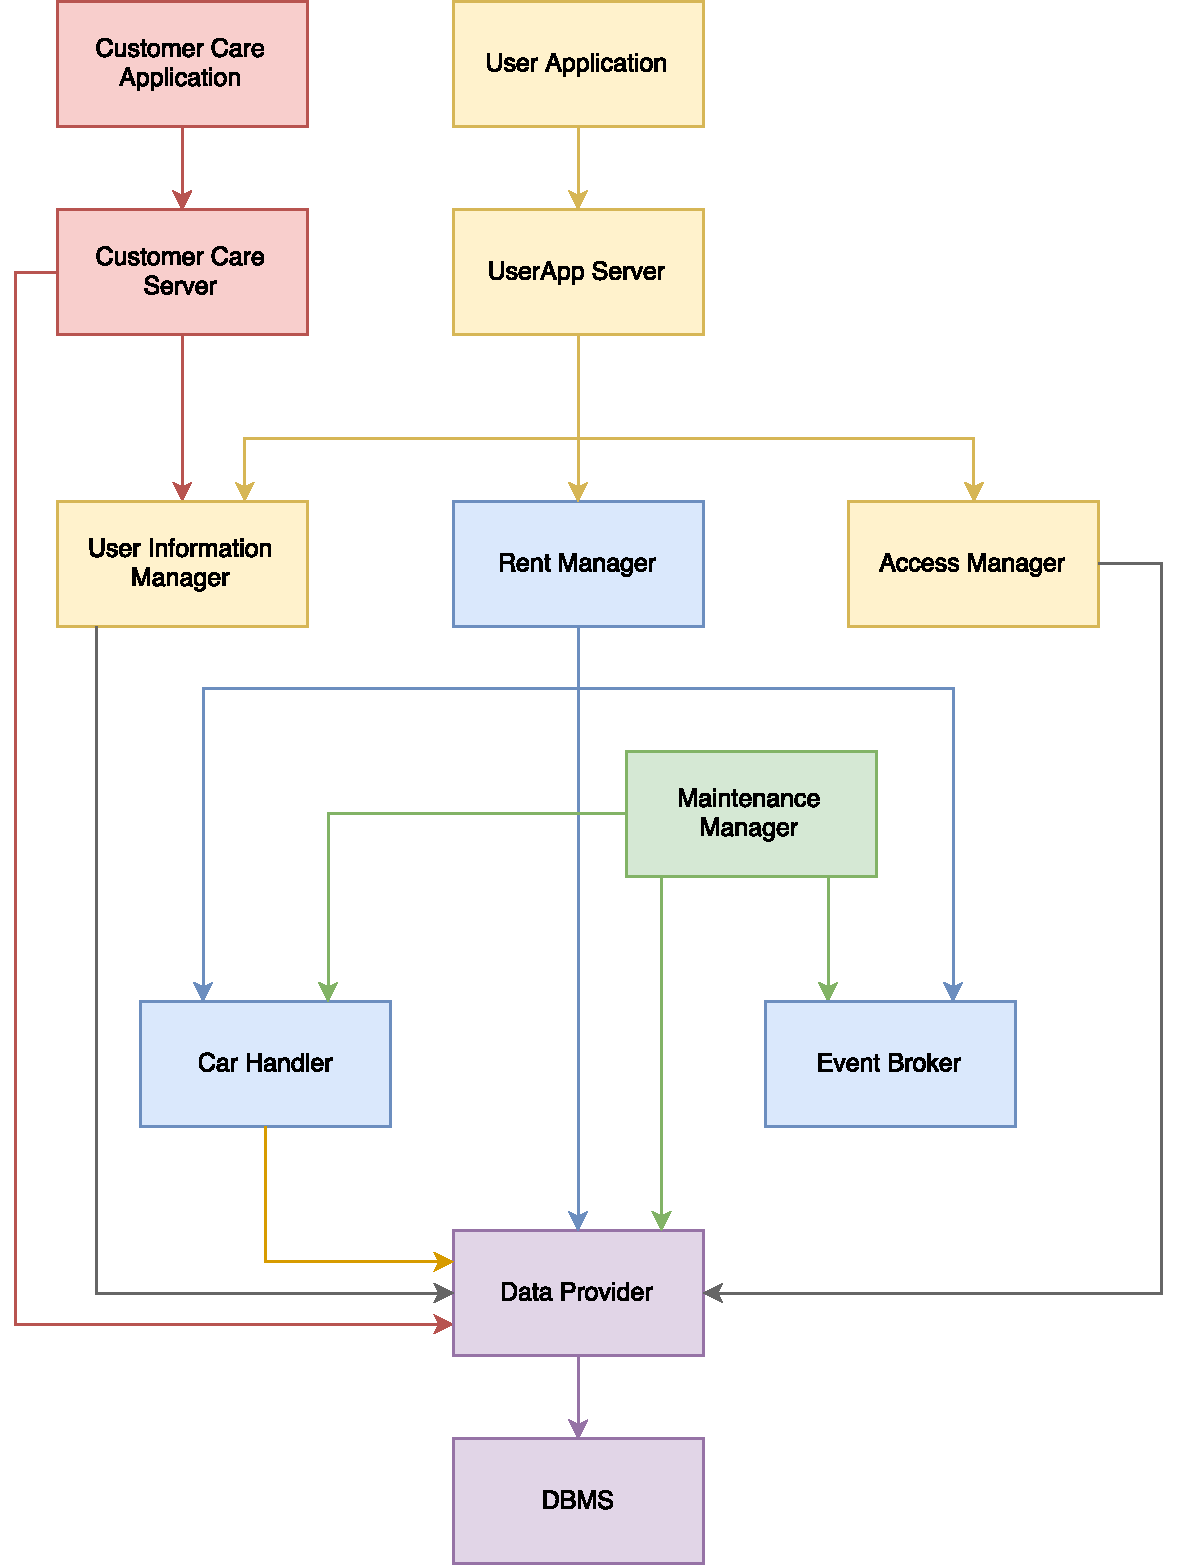
\includegraphics[width=0.8\linewidth]{img/subsystemIntegration}
			\caption{
				\label{fig:subsystemIntegration} 
				\emph{Subsystems Integration}
			}
		\end{figure}
